\documentclass{standalone}
\usepackage{tikz}
\usepackage{ctex,siunitx}
\usepackage{tkz-euclide}
\usepackage{amsmath}
\usetikzlibrary{patterns,calc}
\usetikzlibrary {decorations.pathmorphing, decorations.pathreplacing, decorations.shapes}
\begin{document}
\small
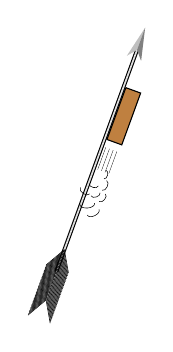
\begin{tikzpicture}[>=latex, scale=1]
  \draw[double=lightgray!50](0,0)--(250:3.0);
  \fill[lightgray](0,0)--(210:0.15)--(70:0.3);
  \fill[gray](0,0)--(290:0.15)--(70:0.3);
  \foreach \x in {2.7,2.72,...,3.4}
  {
    \draw[very thin](250:\x)--++(220:0.3);
    \draw[very thin](250:\x)--++(280:0.3);
  }
  \draw[fill=brown]([shift=(-20:0.03)]250:0.5)--++(250:0.7)--++(-20:0.2)--++(70:0.7)--++(160:0.2);
  \foreach \x in {0.05,0.1,0.15,0.2}
  {
    \draw[ultra thin]([shift=(-20:\x)]250:1.3)--++(250:0.3);
  }
  \begin{scope}[scale=0.5,shift=(250:1.8)]
  \foreach \x/\y/\w/\z in {
    -0.226/-1.584/-0.169/-1.368,
  -0.598/-1.709/-0.371/-1.765,
  -0.827/-1.802/-0.590/-1.968,
  -0.841/-2.229/-0.462/-2.200,
  -0.650/-2.503/-0.351/-2.359,
  -0.347/-2.160/-0.188/-1.969,
  -0.552/-2.016/-0.325/-1.939,
  -0.271/-1.874/-0.158/-1.629}
  {
    \draw[very thin](\x,\y)to[bend right=90](\w,\z);
  }
  \end{scope}
\end{tikzpicture}
\end{document}